\documentclass[xcolor=dvipsnames]{beamer}

% include required packages
\usepackage[sc,slantedGreek]{mathpazo}
\usepackage{helvet}
\usepackage{courier}
\usepackage[T1]{fontenc}
\usepackage{textcomp}

\usepackage{amssymb}
\usepackage{mathtools}
\usepackage{bm}

\usepackage{listings}

\usepackage{pgf}
\usepackage{graphicx}

\usepackage{circuitikz}

\usepackage{tikz}
\usetikzlibrary{arrows,backgrounds,shapes.geometric}

\usepackage{multimedia}

\usepackage{siunitx}


%\usepackage[tagged, highstructure]{accessibility}
\newcommand{\LRT}[2]{\mathrel{\mathop\gtrless\limits^{#1}_{#2}}}
\newcommand{\D}{\mathcal{D}}


\DeclareSIUnit{\sample}{S}


% commands and operators
\DeclareMathOperator{\E}{\bm{E}}
\DeclareMathOperator{\Var}{\bm{Var}}
\DeclareMathOperator*{\argmin}{arg\,min}


% tweak beamer's appeance
\mode<presentation>
{
  \usetheme{Malmoe}
  \usecolortheme[named=ForestGreen]{structure}
  \useoutertheme[footline=authortitle,subsection=false]{miniframes}
}

\mode<handout>
{
  %\beamertemplatesolidbackgroundcolor{black!5}
}

% \AtBeginPart{\frame{\partpage}}

\AtBeginLecture{\frame{\Large Lecture: \insertlecture}}

% \AtBeginSection[]
% {
%   \begin{frame}
%     \frametitle{Outline}
%     \tableofcontents[hideallsubsections]
%   \end{frame}
% }

% document parameters

\title[Practical Methods for Joint Synchronization]
{Practical Methods for Joint Time and Carrier Synchronization in LPI/LPD Communications}
\author[\copyright 2022, HT Zhai and B.-P. Paris]{Haotian Zhai and Dr. B.-P. Paris \\ Dept. Electrical and Comp. Engineering \\ George Mason University}
%\date{Last updated: \today}
\date{November 30, 2022}

\begin{document}

% tweak footer to show page numbers in handouts
\mode<presentation>
{
  % \setbeamercolor{author in head/foot}{fg=black,bg=white}
  % \setbeamercolor{title in head/foot}{fg=black,bg=white}
  % \setbeamercolor{section in head/foot}{fg=black,bg=white}
  % \setbeamercolor{subsection in head/foot}{fg=black,bg=white}
  \setbeamercolor{lower separation line head}{bg=Goldenrod}
  % \setbeamercolor{upper separation line foot}{bg=Goldenrod}


  \setbeamertemplate{footline}
  {%
    \leavevmode%
    \hbox{\begin{beamercolorbox}[wd=.5\paperwidth,ht=2.5ex,dp=1.125ex,leftskip=.3cm,rightskip=.3cm plus1fill]{author in head/foot}%
        \usebeamerfont{author in head/foot}\insertshortauthor
      \end{beamercolorbox}%
      \begin{beamercolorbox}[wd=.5\paperwidth,ht=2.5ex,dp=1.125ex,leftskip=.3cm,rightskip=.3cm plus1fil]{title in head/foot}%
        \usebeamerfont{title in head/foot}\insertshorttitle\hfill\insertframestartpage
      \end{beamercolorbox}}%
    \vskip0pt%
  }
}

% style display boxes
\setbeamercolor{theorem}{fg=blue,bg=lightgray}

% tweak listing's
\lstset{language=Python,basicstyle={\scriptsize\ttfamily},numbers=none,
  numberstyle=\tiny,stepnumber=5,showspaces=false}
\renewcommand{\thelstlisting}{}

% siunitx stuff
% \DeclareSIUnit \belm {bm} % \deci \belm for dBm
% \DeclareSIUnit \belW {bW} % \deci \belW for dBW


% where we keep figures and images
\graphicspath{{../main_matlab_figures/}{../matlab/}}

\logo{
\includegraphics[height=10ex]{mason_logo.png}} 

% boiler plate stuff

\begin{frame}
  \titlepage%
\end{frame}


% \input{050_amplitude_estimation}

% \input{060_initial_acquisition}

% \input{070_PLL}

% \input{080_synch_in_5g}

\section{Agenda}

\begin{frame}
  \frametitle{Agenda}
    \begin{itemize}
        \item{Motivation}
        \item{Prior Work}
        \item{Research Contributions} 
        \begin{itemize}
            \item Joint synchronization algorithm
                \begin{itemize}
                \item Signal model
                \item Time synchronization
                \item Carrier synchronization
                \item Simulation results
                \end{itemize}
            \item Real-time implementation
                \begin{itemize}
                \item Task system
                \item Software-define radio
                \item Flow graph analyzer
                \item Google Benchmark measurement
                \end{itemize}
        \end{itemize}
        \item{Conclusion and Future Work}
    \end{itemize}
\end{frame}

\section{Problem Statement}

% \subsection{Motivation}

\begin{frame}
  \frametitle{Motivation}
  \begin{itemize}
    \item Protecting information in contested and congested wireless communication environments requires transmissions that are difficult to intercept or even detect (LPI/LPD). 
     \item A key measure to achieve robust protection against detection is to rely on signals with power spectral densities that are well below the noise floor. 
     % \item To recover the signals at low SNR, joint detection and carrier synchronization algorithms play a vital role in protected communication system. 
     \item At low SNR, the time and carrier synchronization are coupled problems: coherent methods for detecting the signal require accurate carrier estimations while data-aided carrier estimation requires the location of the training sequence is available.
     \item In practice, the position of the embedded training sequence (preamble) should be searched sequentially.
 
 \end{itemize}
\end{frame}

% \subsection{Previous Work}

\begin{frame}
    \frametitle{Previous Work}
    \begin{itemize}
        \item Some classical works on carrier synchronization were discussed by assuming time synchronization has been accomplished~\cite{Morelli_Mengali_98}. However, this is not reliable especially at low SNR.
        \item The time and carrier synchronization were performed jointly with good accuracy at low SNR in~\cite{purushothaman_16,kim_17}. However, they were doing frame synchronization and the relative
        computation is high.
        \item Computational complexity is another major concern with the practical realization of a synchronization system discussed in~\cite{murin_16,wang_21}.
    
    \end{itemize}
  \end{frame}



\begin{frame}
    \frametitle{Our Research}
    \begin{itemize}
        \item Our research provides a comprehensive treatment of the signal acquisition problem of protected communications, which basically includes
        \begin{itemize}
            \item a family of joint detection and estimation algorithm that emphasize computational complexity while maintaining near-optimal accuracy at very low SNR, and
            \item the implementation of the proposed algorithms on a standard SDR platform.
        \end{itemize} 
    \end{itemize}

    \begin{figure}
        \centering
        \begin{minipage}{.5\textwidth}
          \centering
          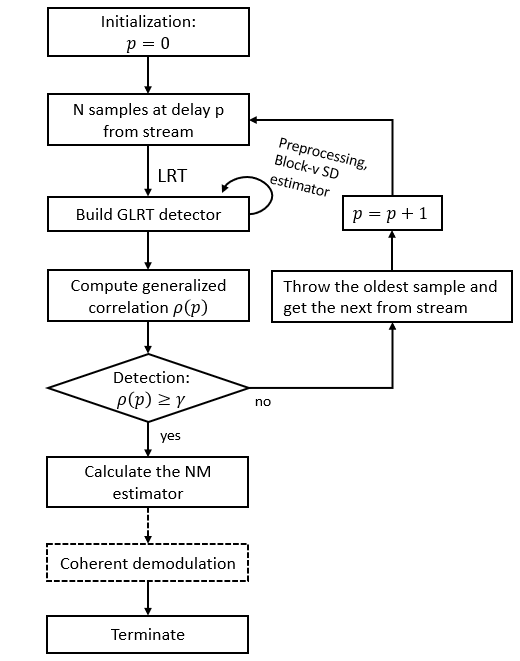
\includegraphics[width=.5\linewidth]{architecture_of_paper.png}
        \end{minipage}%
        \begin{minipage}{.5\textwidth}
          \centering
          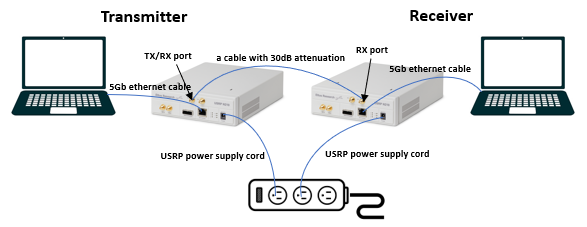
\includegraphics[width=.8\linewidth]{SDR_signal_transmission_path.png}
        \end{minipage}
    \end{figure}

\end{frame}



\section{Theoretical explanation}

\subsection{Signal Model}

\subsection{Time Synchronization}

\begin{frame}
    \frametitle{Time synchronization}

    \begin{center}
      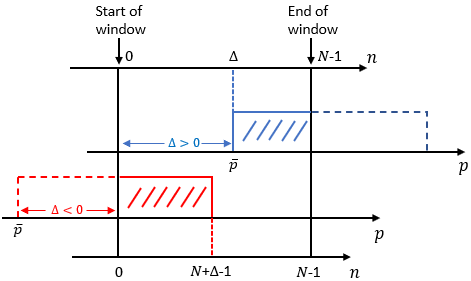
\includegraphics[width=.38\textwidth]{partial_preamble_detection.png}
    \end{center}

    \begin{itemize}
      \item Two hypotheses for sequential detection task are given by:
      
      \begin{equation}
        \label{eq:two hypotheses}
        \begin{aligned}
        &H_0{:}~r_n{=}
        \begin{dcases}
            s_{n-\Delta}\xi e^{j2\pi\delta (n-\Delta)}{+}w_n & \max(0{,}\Delta){\leq} n {<} \min(N{,}N{+}\Delta) \\
            w_n & \text{otherwise},
        \end{dcases} \\
        &H_1{:}~r_n{=}s_n\xi e^{j2\pi\delta n}+w_n,
        \end{aligned}
      \end{equation}
      where
      
      \begin{itemize}
          % \item $H_0$: the received signal is the channel noise or only contains a portion of the preamble.
          % \item $H_1$: the received signal contains the entire preamble.
          \item $\Delta$ is the distance between the current start position of the observation window and the true position of the preamble $\bar{p}$.
      \end{itemize}

    \end{itemize} 

\end{frame}


\begin{frame}
    \frametitle{Hypothesis Testing}
    \begin{itemize}

      \item The conditional likelihood ratio test (CLRT) is built by conditioning on $\Delta$, the phasor $\xi$, and the frequency offset $\delta$
  
      \begin{equation}
          \label{eq:log likelihood}
          \begin{aligned}
          \Re\Bigg\{\sum_{n=0}^{N-1}r_ns_n^*\xi^*e^{-j2\pi\delta n}-\sum_{n=\Delta}^{N-1}r_n&s_{n-\Delta}^*\xi^*e^{-j2\pi\delta(n-\Delta)}\Bigg\} \LRT{H_1}{H_0} \\
          &\frac{N_0}{2}\ln\eta+\frac{A^2}{2}\sum_{n=N-\Delta}^{N-1}|s_n|^2.
          \end{aligned}
      \end{equation}
  
      \begin{itemize}
          \item The two inner products on left hand side are the matched filters for hypothesis $H_1$ and $H_0$.
          \item The matched filter for $H_0$ is not computable in practice due to the unknown information of $\Delta$.
          \item The effect of the partial correlation can be neglected by using a preamble with very good autocorrelation property.
      \end{itemize}
      
  \end{itemize}

\end{frame}

\begin{frame}
  \frametitle{The Sequential Detector}
    \begin{itemize}
    
        \item A practical sequential detector is given based on the above discussion for each observation window at global sample index $p$
        \begin{equation}
          \label{eq:generalized_corr}
          \rho(p)=
          \frac{\Re\{\langle
            \boldsymbol{r}_{p},\hat{\boldsymbol{s}}_{p}\rangle\}}
          {||\boldsymbol{r}_{p}||\cdot||\hat{\boldsymbol{s}}_{p}||} \LRT{H_1}{H_0} \gamma
        \end{equation}

        where 
        \begin{itemize}
          \item $\bm{r}_{p}{=}[r_{p},r_{p+1},\ldots,r_{p+N-1}]$ denotes the received signal in the observation window
          starting at position $p$.
          \item $\hat{\bm{s}}_{p}$ denotes the carrier-corrected preamble,
          where each element is $\hat{s}_{n}=s_n\hat{\xi}_{p}e^{j2\pi\hat{\delta}_{p}n}$
          for $n=0,1,\ldots,N{-}1$, and $\hat{\xi}_{p}$, $\hat{\delta}_{p}$ are the carrier estimates at
          position $p$.
          \item A realistic generalized likelihood ratio test (GLRT) replaces the CLRT.
          \item The complexity of estimating $\hat{\xi}$,$\hat{\delta}$ is critical for practical implementation. 

        \end{itemize}
        
        
    \end{itemize}

\end{frame}

\subsection{Carrier Synchronization}

\begin{frame}
  \frametitle{Carrier Synchronization}
    \begin{itemize}
    
       \item Assume that the time synchronization is perfect.
       \item The maximum likelihood estimation (MLE) of the parameters in the signal model is given by
       
       \begin{equation}
        \label{eq:ML_f_xi}
        \hat{\delta},\hat{\xi}=\min_{\delta,\xi=Ae^{j\phi}}\sum_{n=0}^{N-1}|r_n-s_n\xi e^{j2\pi\delta n}|^{2}.
      \end{equation}

      \item The closed form for $\hat{\xi}$ and a necessary condition for $\hat{\delta}$ are obtained by taking the Wirtinger derivative
      
      \begin{equation}
        \label{eq:opt_xi}
        \hat{\xi}=\frac{\sum_{n=0}^{N-1}{r_{n}s_n^{*}e^{-j2\pi\hat{\delta} n}}}{\sum_{n=0}^{N-1}|s_{n}|^2},
      \end{equation}

      \begin{equation}
        \label{eq:necessary condition for delta}
        J(\hat{\delta}) = \Im\bigg\{\sum_{k=1}^{N-1}{\sum_{m=k}^{N-1}{kr_{m-k}r_m^{*}s_{m-k}^{*}s_m}e^{j2\pi\hat{\delta}k}}\bigg\}=0.
      \end{equation}

    \end{itemize}


\end{frame}


\begin{frame}
  \frametitle{Coarse Estimator: Single-Lag Estimator with Partial Coherent Integration}

    \begin{itemize}
    
      \item At moderate SNR, every lag $k$ can be used to approximate the frequency estimate $\delta$. This suggests that an unbiased estimate of $\delta$ can be obtained by using only a single lag $k$.
      \item To extend the operation to low SNR, a generalized SL estimator with PCI is derived
      
      \begin{equation}
        \label{eq:single_lag_estimator_w_partial_corr}
        \hat{\delta}_{SL}^{(v)}(k_v)=-\frac{\arg\big\{\sum_{l=k_v}^{N/v-1}\digamma_l^{*(v)}\digamma_{l-k_v}^{(v)}\big\}}{2\pi k_vv},
      \end{equation}

      where $\digamma_{l}^{(v)}$ is the result of PCI over block $l$
      of length $v$

      \begin{equation}
        \label{eq:coherent_integrator}
        \digamma_l^{(v)}=\sum_{n=lv}^{(l+1)v-1}r_ns_n^*, \quad \text{for}~l=0,1,\ldots,N/v{-}1.
      \end{equation}

      \begin{itemize}
        \item  $k_v=\lfloor k/v \rfloor$.
      \end{itemize}

    \end{itemize}

    % \begin{center}
    %   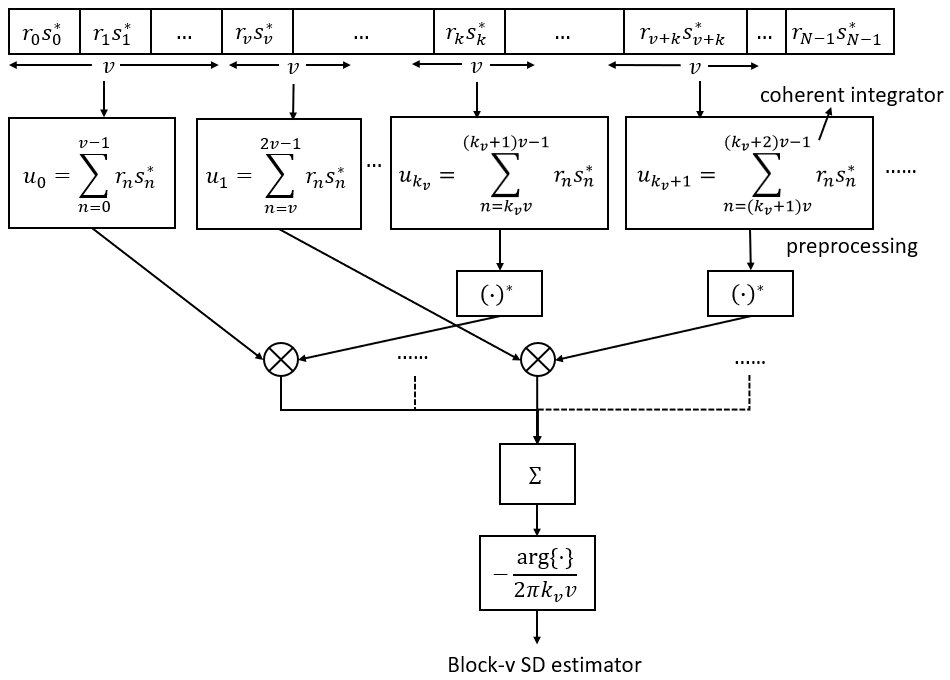
\includegraphics[width=.5\textwidth]{general_SD_estimator.png}
    % \end{center}


\end{frame}



\begin{frame}
  \frametitle{Block diagram}

    \begin{center}
      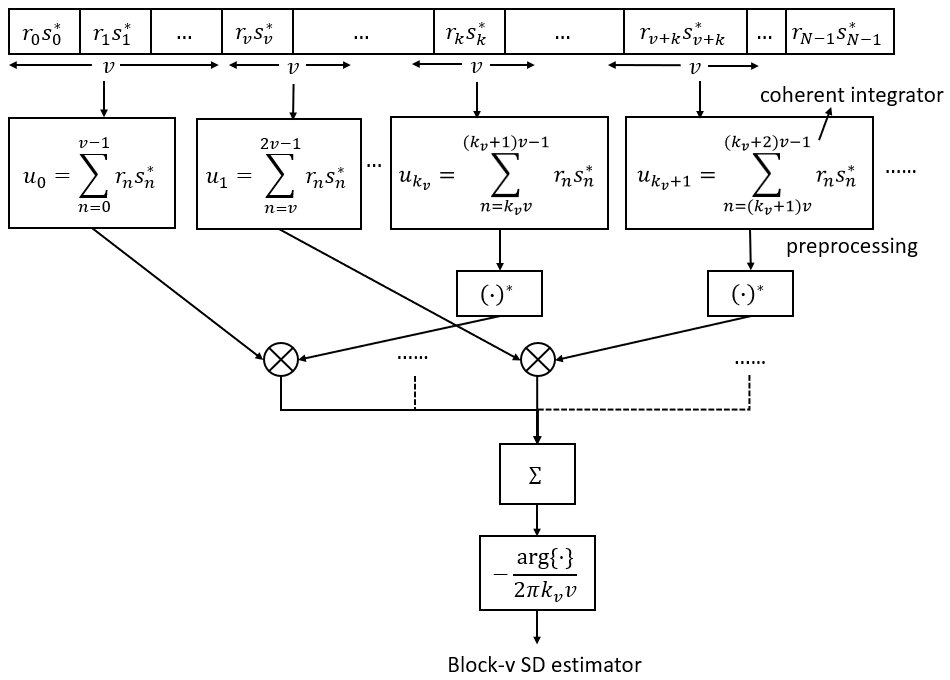
\includegraphics[width=.5\textwidth]{general_SD_estimator.png}
    \end{center}

    \begin{itemize}
    
      \item The above figure illustrates how Single-Lag estimator with PCI works.
      \item The intention of PCI is to increase the SNR of coherent terms before estimating frequency offset from non-coherent terms by leveraging the processing gain.
      \item The complexity is degraded by $O(N)$.

    \end{itemize}

    % \begin{center}
    %   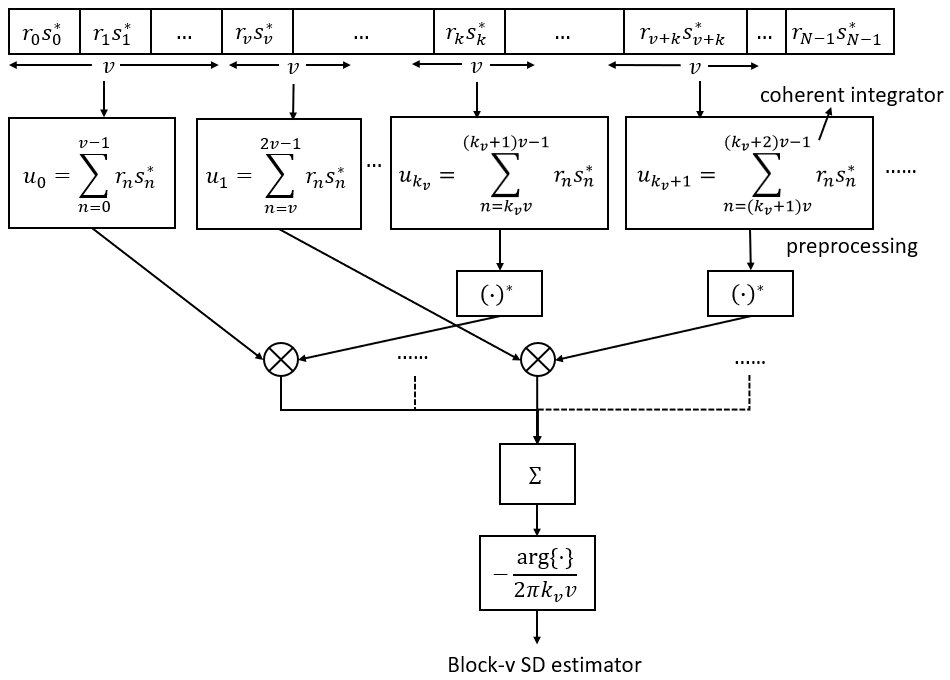
\includegraphics[width=.5\textwidth]{general_SD_estimator.png}
    % \end{center}


\end{frame}


\begin{frame}
  \frametitle{Probability distribution over non-coherent blocks}

    \begin{itemize}
    
      \item Define $C_{\digamma}(v,l)=\digamma_l^*\digamma_{l-k_v}$ and it has a mixed distribution of a complex Gaussian and 
      a Bessel function of the second kind (from noise), whose mean and variance are

      \begin{equation}
        \begin{aligned}
        \label{eq:mean_var_product_coherent_int}
        \mu_{C_{\digamma}}&=\frac{E_s}{M}\sum_{n=lv}^{(l+1)v-1}e^{-j2\pi \delta n}\bigg(\sum_{m=(l-k_v)v}^{(l-k_v+1)v-1}e^{j2\pi \delta m}\bigg) \\
        &=E_s/M\cdot e^{-j2\pi \delta k_vv}\D^2(v,\delta), \\
        \sigma^2_{C_{\digamma}}&={\underbrace{N_0^2v^2/4}_{\text{from Bessel}}}+{\underbrace{N_0E_sv/M\cdot\D^2(v,\delta)}_{\text{from Complex Gaussian}}},
        \end{aligned}
      \end{equation}

      where 
      \begin{itemize}
        \item $\D(v,\delta) = \frac{\sin(\pi \delta v)}{\sin(\pi
        \delta)}$ is the Dirichlet function of $\delta$, which approaches 
        the maximum value $v$ at $\delta=0$.
      \end{itemize}


    \end{itemize}

    % \begin{center}
    %   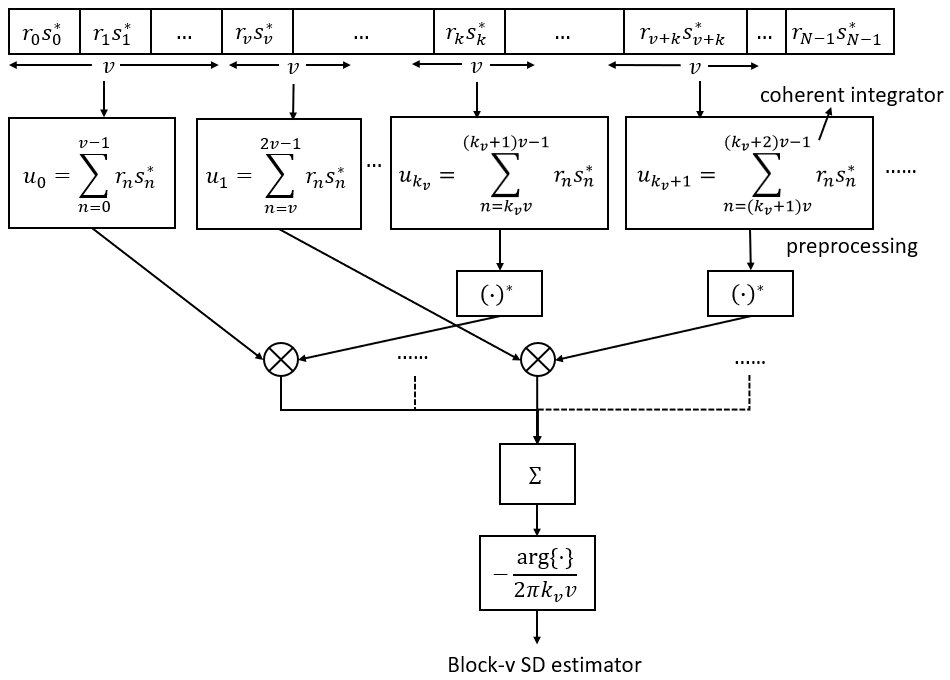
\includegraphics[width=.5\textwidth]{general_SD_estimator.png}
    % \end{center}


\end{frame}


\begin{frame}
  \frametitle{Performance improvement by PCI}

    \begin{itemize}

      \item One way to look at the performance of the SL estimator with PCI is by the "output" SNR
      
      \begin{equation}
        \begin{aligned}
          \label{eq:SNR_out}
          \text{SNR}_{\sum C_{\digamma}}^{(v,\delta)}=\frac{|\mu_{\sum C_{\digamma}}|^2}{\sigma^2_{\sum C_{\digamma}}} 
          =\frac{(N/v-k_v)\cdot\D^4(v,\delta)}
          {v^2/\text{SNR}_{\text{in}}+2v\cdot\D^2(v,\delta)}\cdot\text{SNR}_{\text{in}}. \\
        \end{aligned}
      \end{equation}
    
      \begin{itemize}
        \item The "output" SNR is degraded by the variance of the second kind Bessel random variable.
      \end{itemize}

      \item To see PCI improves the performance of SL at low SNR via the ratio
      
      \begin{equation}
        \begin{aligned}
          \label{eq:relative_processing_gain}
          \frac{\text{SNR}_{\sum C_{\digamma}}^{(v,0)}}{\text{SNR}_{\sum C_{\digamma}}^{(1,0)}}
          \approx\frac{v+2v\cdot\text{SNR}_{\text{in}}}{1+2v\cdot\text{SNR}_{\text{in}}}.
        \end{aligned}
      \end{equation}

      \begin{itemize}
        \item the relative performance increases with $v$ at very low SNR.
      \end{itemize}

    \end{itemize}

    % \begin{center}
    %   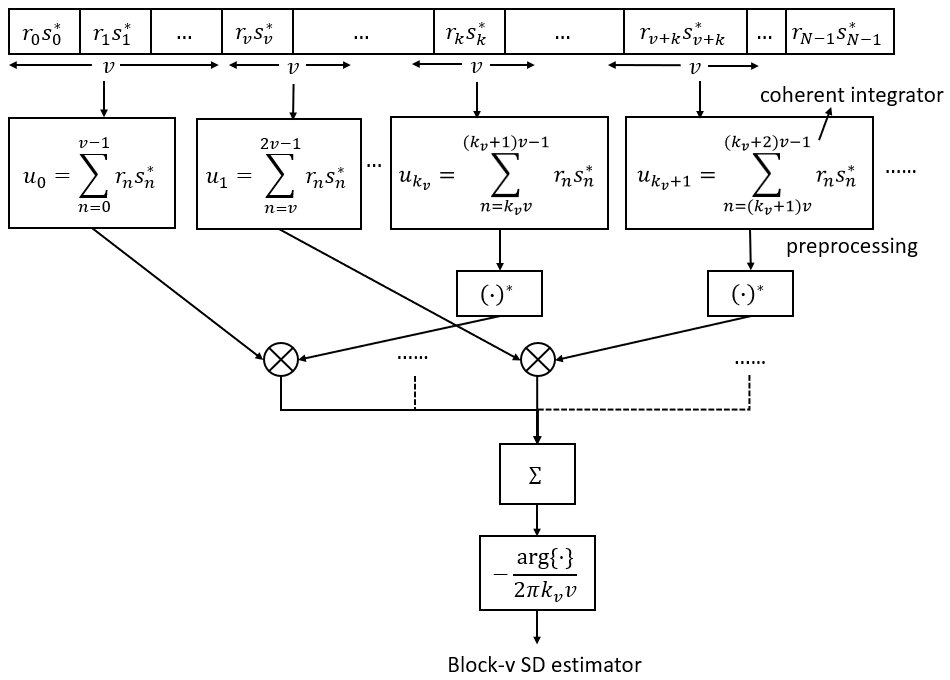
\includegraphics[width=.5\textwidth]{general_SD_estimator.png}
    % \end{center}


\end{frame}


\begin{frame}
  \frametitle{Fine Estimator: Newton-Method based Estimator}

    \begin{itemize}
    
      \item Use the SL estimator as starting point for a Newton-type iteration aimed at finding a better solution to the necessary condition for $\hat{\delta}$ in~\eqref{eq:necessary condition for delta}
      
      \begin{equation}
        \label{eq:iter_NM_est}
        \hat{\delta}_{NM}^{(i+1)}=\hat{\delta}_{NM}^{(i)}-
        \frac{J(\hat{\delta}_{NM}^{(i)})}{J^\prime(\hat{\delta}_{NM}^{(i)})}
      \end{equation}

      \begin{itemize}
        \item $\hat{\delta}_{NM}^{(0)}=\hat{\delta}^{(v)}_{SL}(k_v)$.
        \item $J^\prime(\cdot)$ is the derivative of $J$ with respect to $\hat{\delta}$.
        \item A single iteration is usually sufficient to achieve very good accuracy.
        \item Complexity is $O(N^2)$.
      \end{itemize}

      \item Summary: The SL estimator is used for operating at high sample rate for sequential detection task due to its low complexity.
      The NM estimator improves the accuracy after reliable detection to enable coherent demodualtion.
        

    \end{itemize}




\end{frame}

\subsection{Simulation}

\begin{frame}
  \frametitle{Simulation Results}

    \begin{center}
      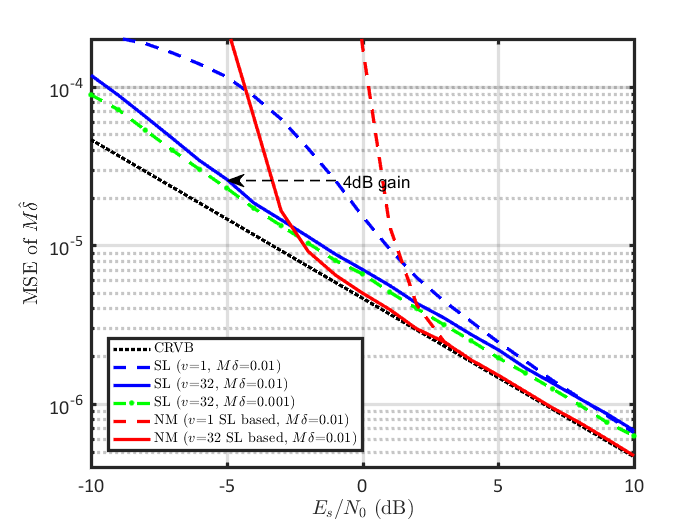
\includegraphics[width=.521\textwidth]{accuracy_NM_SL_slides.png}
    \end{center}

    \begin{itemize}
    
      \item The accuracy is improved from SL w/o PCI at $\SI{-1}{\dB}$ to with PCI at $\SI{-5}{\dB}$ by $\SI{4}{\dB}$ gain, which is consistent with~\eqref{eq:relative_processing_gain}.
      \item The accuracy of SL is higher at all SNRs with lower frequency offset because of the Derichlet function.  
      \item NM approaches the CRVB as SL reaches some accuracy.

    \end{itemize}




\end{frame}

\begin{frame}
  \frametitle{Simulation Results}

    \begin{center}
      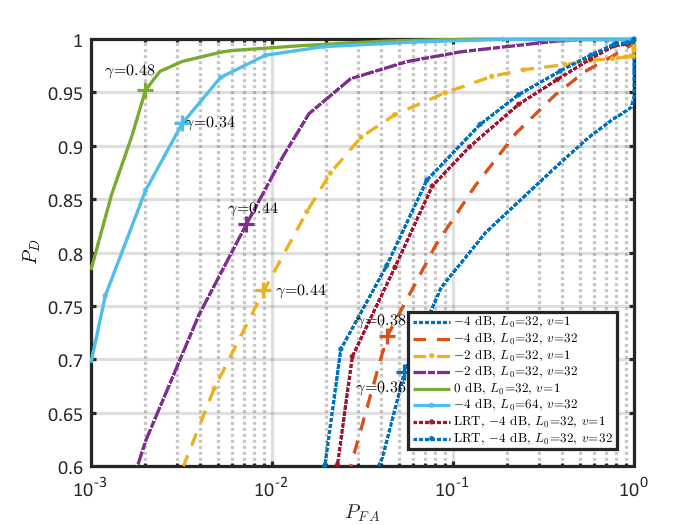
\includegraphics[width=.521\textwidth]{ROC_new.png}
    \end{center}

    \begin{itemize}
    
      \item The above figure shows the receiver operating characteristics (ROC) of the sequential detector.
      \item The better accuracy of SL with PCI also improves the detection performance at low SNR.
      \item The performance can also be significantly improved by leveraging a larger size of the preamble.

    \end{itemize}

\end{frame}

\section{Real-time Implementation}

% agenda maybe changed a bit.

% fga, throughput and latency, accuracy
% benchmark, throughput
% demo or a picture.

\begin{frame}
    \frametitle{Task Based Signal Processing System}

    \begin{columns}
      \begin{column}{0.515\textwidth}
        
        \begin{itemize}
          \item Using a task based digital signal processing system at the receiver 
          \begin{itemize}
              \item Each function maps to an individual task. 
              \item Tasks are processed in parallel if no data dependency occurs.             
             
          \end{itemize} 
          \item Different aspects of the algorithm are mapped in 
          a pipelined, parallel task processing architecture via Threading Building Blocks~\cite{Michael_19}. 


        \end{itemize}

      \end{column} 

    \begin{column}{0.46\textwidth} 

        \begin{center}
          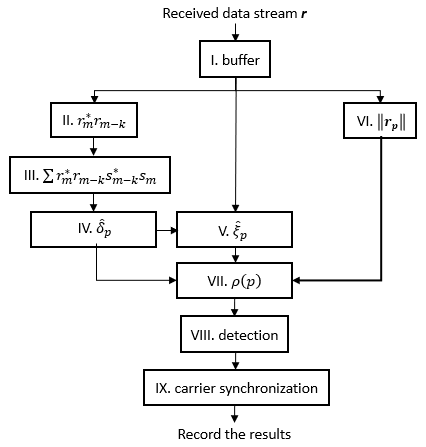
\includegraphics[width=1.0\linewidth]{SDR_receiver_new_slides.png}
        \end{center}
      
      \end{column}
    \end{columns}

    % \begin{figure}
    %     \centering
    %     \begin{minipage}{.5\textwidth}
    %       \centering
    %       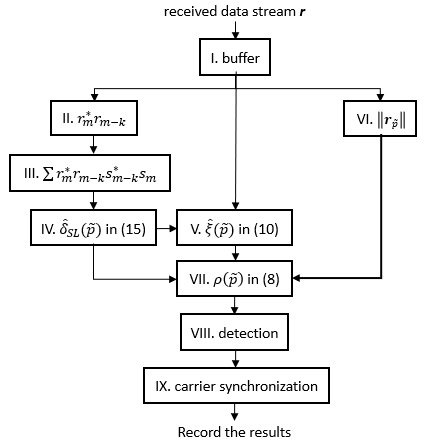
\includegraphics[width=.5\linewidth]{SDR_receiver_new.png}
    %     \end{minipage}%
    %     \begin{minipage}{.5\textwidth}
    %       \centering
    %       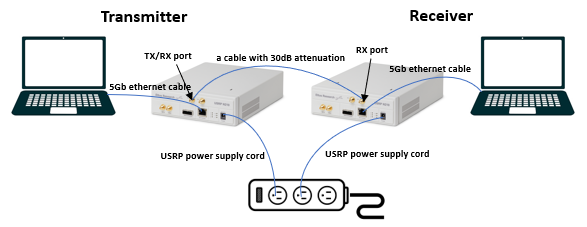
\includegraphics[width=.8\linewidth]{SDR_signal_transmission_path.png}
    %     \end{minipage}
    % \end{figure}

    % \begin{itemize}
    %     \item Different aspects of our algorithm are mapped to logical nodes in a pipelined, parallel processing architecture using Threading Building Blocks (TBB).
    %     \item The signals are transmitted and received between two universal software radio peripherals (USRP) connected by 5 Gb/s Ethernet cables to
    %     laptops.
    %     \item Accuracy, throughput and latency (the time when the first joint detection and estimation are finished) are considered. 
    % \end{itemize}
  \end{frame}


  \begin{frame}
    \frametitle{Software-defined Radio}
    \begin{center}
      \includegraphics[width=.8\textwidth]{SDR_real.jpeg}
    \end{center}

  \end{frame} 


  \begin{frame}
    \frametitle{Flow Graph Analyzer~\cite{Intel_Corporation}: Latency and Throughput}

    % need more explain on how FGA works.

    \begin{figure}
        \centering
          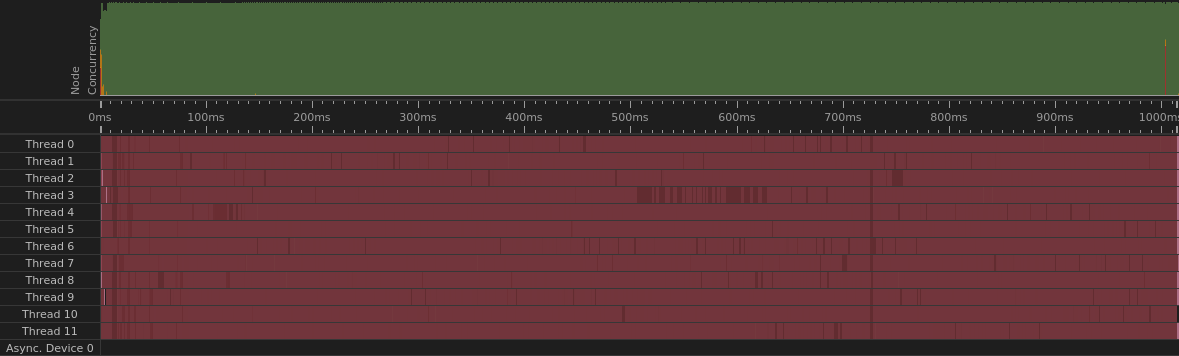
\includegraphics[width=.62\linewidth]{fga_throughput.png}
    \end{figure}

    \begin{figure}
      \centering
        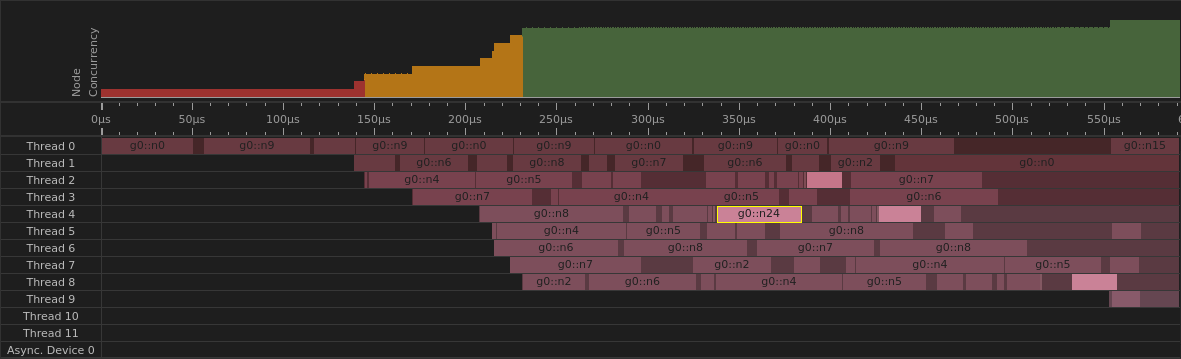
\includegraphics[width=.62\linewidth]{fga_latency.png}
  \end{figure}

    \begin{itemize}
        \item The top graph shows that the task based implementaton
          exhibits high parallelism; all cores are used.
          \begin{itemize}
          \item The throughput is approximately
            $ \SI[per-mode=symbol]{28.74}{\mega\sample\per\second}$.
          \end{itemize}
        \item By zooming in on the start of processing, the latency (finish time of the first burst) is observed around $ \SI[per-mode=symbol]{383.7}{\nano\second}$.

    \end{itemize}
  \end{frame}


  \begin{frame}
    \frametitle{Google Benchmark: Task Duration Measurement}

    \begin{figure}
        \centering
        \begin{table}[t]
          \tiny
          \centering % used for centering table
          \begin{tabular}{c c c c} % centered columns (4 columns)
          \hline\hline %inserts double horizontal lines
          Node name & Time (ns) & CPU (ns) & Iterations \\ [0.5ex] % inserts table
          %heading
          \hline % inserts single horizontal line
          I. Buffer  & 3487 & 3487 & 206840 \\ % inserting body of the table
          II. $r_m^*r_{m-k}$  & 3530 & 3530 & 198687 \\
          III. $r_m^*r_{m-k}s_{m-k}^*s_m$ & 49290 & 49289 & 13958 \\
          IV. $\hat{\delta}_{SL}^{(1)}$ & 53219 & 53217 & 12180 \\
          V. $\hat{\xi}$ & 65397 & 65388 & 15312 \\
          VI. $||\bm{r}||$ & 13130 & 13129 & 52026 \\ % [1ex] adds vertical space
          VII. $\rho(p)$ & 7278 & 7278 & 92031 \\
          VIII. detection & 5521 & 5521 & 123079 \\
          IX. carrier synchronization & 46855 & 46851 & 14867  \\ [1ex]
          \hline
          \end{tabular}
          \label{table:BM_function_nodes} % is used to refer this table in the text
        \end{table}   
    \end{figure}

    \begin{itemize}
       \item Benchmark each task of proposed algorithm
         (\qty{2048}{\sample} input):
       \begin{itemize}
        \item measure the throughput that each task can achieve
        \item identify the task with the longest duration for
          potential increase of throughput of he entire system
       \end{itemize}
       \item The throughput is bounded by slowest block, $\SI{2048}{\sample}/\SI{65397}{\nano\second}  \approx \SI[per-mode=symbol]{31.32}{\mega\sample\per\second}$.
    \end{itemize}
  \end{frame}

 


  \begin{frame}
    \frametitle{Summary and Future Work}
    \begin{itemize}
      \item A family of algorithms for joint detection and carrier synchronization for LPI/LPD communications was presented.
      \begin{itemize}
        \item The algorithm is designed for low complexity while achieving good performance over a wide range of SNR.
      \end{itemize}
      \item The real-time practicality of the algorithm is validated via a software-defined radio platform.
      \begin{itemize}
        \item Different aspects of algorithm are mapped in a highly pipelined and parallel task architecture.
      \end{itemize}
      \item Extend the proposed algorithm for dispersive channels.
      \item Package the C++ code of real-time implementation as the open source distribution.
    \end{itemize}
      
  \end{frame} 


\bibliographystyle{ieeetr}
\bibliography{ref.bib}

\end{document}
